\documentclass{beamer}

% xcolor and define colors -------------------------
\usepackage{xcolor}

% https://www.viget.com/articles/color-contrast/
\definecolor{purple}{HTML}{5601A4}
\definecolor{navy}{HTML}{0D3D56}
\definecolor{ruby}{HTML}{9a2515}
\definecolor{alice}{HTML}{107895}
\definecolor{daisy}{HTML}{EBC944}
\definecolor{coral}{HTML}{F26D21}
\definecolor{kelly}{HTML}{829356}
\definecolor{cranberry}{HTML}{E64173}
\definecolor{jet}{HTML}{131516}
\definecolor{asher}{HTML}{555F61}
\definecolor{slate}{HTML}{314F4F}

% Mixtape Sessions
\definecolor{picton-blue}{HTML}{00b7ff}
\definecolor{violet-red}{HTML}{ff3881}
\definecolor{sun}{HTML}{ffaf18}
\definecolor{electric-violet}{HTML}{871EFF}

\newcommand\pictonBlue[1]{{\color{picton-blue}#1}}
\newcommand\sun[1]{{\color{sun}#1}}
\newcommand\electricViolet[1]{{\color{electric-violet}#1}}
\newcommand\violetRed[1]{{\color{violet-red}#1}}

\newcommand\bgPictonBlue[1]{{\colorbox{picton-blue!20!white}{#1}}}
\newcommand\bgSun[1]{{\colorbox{sun!20!white}{#1}}}
\newcommand\bgElectricViolet[1]{{\colorbox{electric-violet!20!white}{#1}}}
\newcommand\bgVioletRed[1]{{\colorbox{violet-red!20!white}{#1}}}

\def\code#1{\texttt{#1}}

% Main theme colors
\definecolor{accent}{HTML}{00b7ff}
\definecolor{accent2}{HTML}{871EFF}
\definecolor{gray100}{HTML}{f3f4f6}
\definecolor{gray800}{HTML}{1F292D}


% Beamer Options -------------------------------------

% Background
\setbeamercolor{background canvas}{bg = white}

% Change text margins
\setbeamersize{text margin left = 15pt, text margin right = 15pt} 

% \alert
\setbeamercolor{alerted text}{fg = accent2}

% Frame title
\setbeamercolor{frametitle}{bg = white, fg = jet}
\setbeamercolor{framesubtitle}{bg = white, fg = accent}
\setbeamerfont{framesubtitle}{size = \small, shape = \itshape}

% Block
\setbeamercolor{block title}{fg = white, bg = accent2}
\setbeamercolor{block body}{fg = gray800, bg = gray100}

% Title page
\setbeamercolor{title}{fg = gray800}
\setbeamercolor{subtitle}{fg = accent}

%% Custom \maketitle and \titlepage
\setbeamertemplate{title page}
{
    %\begin{centering}
        \vspace{20mm}
        {\Large \usebeamerfont{title}\usebeamercolor[fg]{title}\inserttitle}\\
        {\large \itshape \usebeamerfont{subtitle}\usebeamercolor[fg]{subtitle}\insertsubtitle}\\ \vspace{10mm}
        {\insertauthor}\\
        {\color{asher}\small{\insertdate}}\\
    %\end{centering}
}

% Table of Contents
\setbeamercolor{section in toc}{fg = accent!70!jet}
\setbeamercolor{subsection in toc}{fg = jet}

% Button 
\setbeamercolor{button}{bg = accent}

% Remove navigation symbols
\setbeamertemplate{navigation symbols}{}

% Table and Figure captions
\setbeamercolor{caption}{fg=jet!70!white}
\setbeamercolor{caption name}{fg=jet}
\setbeamerfont{caption name}{shape = \itshape}

% Bullet points

%% Fix spacing between items
\let\olditemize=\itemize 
\let\endolditemize=\enditemize 
\renewenvironment{itemize}{\vspace{0.25em}\olditemize \itemsep0.25em}{\endolditemize}

%% Fix left-margins
\settowidth{\leftmargini}{\usebeamertemplate{itemize item}}
\addtolength{\leftmargini}{\labelsep}

%% enumerate item color
\setbeamercolor{enumerate item}{fg = accent}
\setbeamerfont{enumerate item}{size = \small}
\setbeamertemplate{enumerate item}{\insertenumlabel.}

%% itemize
\setbeamercolor{itemize item}{fg = accent!70!white}
\setbeamerfont{itemize item}{size = \small}
\setbeamertemplate{itemize item}[circle]

%% right arrow for subitems
\setbeamercolor{itemize subitem}{fg = accent!60!white}
\setbeamerfont{itemize subitem}{size = \small}
\setbeamertemplate{itemize subitem}{$\rightarrow$}

\setbeamertemplate{itemize subsubitem}[square]
\setbeamercolor{itemize subsubitem}{fg = jet}
\setbeamerfont{itemize subsubitem}{size = \small}








% Links ----------------------------------------------

\usepackage{hyperref}
\hypersetup{
  colorlinks = true,
  linkcolor = accent2,
  filecolor = accent2,
  urlcolor = accent2,
  citecolor = accent2,
}


% Line spacing --------------------------------------
\usepackage{setspace}
\setstretch{1.35}


% \begin{columns} -----------------------------------
\usepackage{multicol}


% Fonts ---------------------------------------------
% Beamer Option to use custom fonts
\usefonttheme{professionalfonts}

% \usepackage[utopia, smallerops, varg]{newtxmath}
% \usepackage{utopia}
\usepackage[sfdefault,light]{roboto}

% Small adjustments to text kerning
\usepackage{microtype}



% Remove annoying over-full box warnings -----------
\vfuzz2pt 
\hfuzz2pt


% Table of Contents with Sections
\setbeamerfont{myTOC}{series=\bfseries, size=\Large}
\AtBeginSection[]{
        \frame{
            \frametitle{Roadmap}
            \tableofcontents[current]   
        }
    }


% Tables -------------------------------------------
% Tables too big
% \begin{adjustbox}{width = 1.2\textwidth, center}
\usepackage{adjustbox}
\usepackage{array}
\usepackage{threeparttable, booktabs, adjustbox}
    
% Fix \input with tables
% \input fails when \\ is at end of external .tex file
\makeatletter
\let\input\@@input
\makeatother

% Tables too narrow
% \begin{tabularx}{\linewidth}{cols}
% col-types: X - center, L - left, R -right
% Relative scale: >{\hsize=.8\hsize}X/L/R
\usepackage{tabularx}
\newcolumntype{L}{>{\raggedright\arraybackslash}X}
\newcolumntype{R}{>{\raggedleft\arraybackslash}X}
\newcolumntype{C}{>{\centering\arraybackslash}X}

% Figures

% \imageframe{img_name} -----------------------------
% from https://github.com/mattjetwell/cousteau
\newcommand{\imageframe}[1]{%
    \begin{frame}[plain]
        \begin{tikzpicture}[remember picture, overlay]
            \node[at = (current page.center), xshift = 0cm] (cover) {%
                \includegraphics[keepaspectratio, width=\paperwidth, height=\paperheight]{#1}
            };
        \end{tikzpicture}
    \end{frame}%
}

% subfigures
\usepackage{subfigure}


% Highlight slide -----------------------------------
% \begin{transitionframe} Text \end{transitionframe}
% from paulgp's beamer tips
\newenvironment{transitionframe}{
    \setbeamercolor{background canvas}{bg=accent!40!black}
    \begin{frame}\color{accent!10!white}\LARGE\centering
}{
    \end{frame}
}


% Table Highlighting --------------------------------
% Create top-left and bottom-right markets in tabular cells with a unique matching id and these commands will outline those cells
\usepackage[beamer,customcolors]{hf-tikz}
\usetikzlibrary{calc}
\usetikzlibrary{fit,shapes.misc}

% To set the hypothesis highlighting boxes red.
\newcommand\marktopleft[1]{%
    \tikz[overlay,remember picture] 
        \node (marker-#1-a) at (0,1.5ex) {};%
}
\newcommand\markbottomright[1]{%
    \tikz[overlay,remember picture] 
        \node (marker-#1-b) at (0,0) {};%
    \tikz[accent!80!jet, ultra thick, overlay, remember picture, inner sep=4pt]
        \node[draw, rectangle, fit=(marker-#1-a.center) (marker-#1-b.center)] {};%
}


% DAGS ----------------------------------------------
\usepackage{tikz}
\usetikzlibrary{shapes,decorations,arrows,calc,arrows.meta,fit,positioning}
% Tikz settings optimized for causal graphs.
\tikzset{
    -Latex,auto,node distance =1 cm and 1 cm,semithick,
    state/.style ={ellipse, draw, minimum width = 0.7 cm},
    point/.style = {circle, draw, inner sep=0.04cm,fill,node contents={}},
    bidirected/.style={Latex-Latex,dashed},
    el/.style = {inner sep=2pt, align=left, sloped}
}


% Beamer tricks -------------------------------------
% Make \pause work in align environments
\makeatletter
\renewrobustcmd{\beamer@@pause}[1][]{%
  \unless\ifmeasuring@%
  \ifblank{#1}%
    {\stepcounter{beamerpauses}}%
    {\setcounter{beamerpauses}{#1}}%
  \onslide<\value{beamerpauses}->\relax%
  \fi%
}
\makeatother




\begin{document}

\imageframe{./lecture_includes/cover_understanding.png}

\section{Where do (Good) Instruments Come From?}

\subsection{True Lotteries}
\begin{frame}{Subtlties of the Validity Condition}

To apply IV, we need to make a good case for instrument validity \\ (note we can always check relevance!)\pause
\medskip

Consider our simple causal model, $Y_i=\alpha+\beta D_i+\varepsilon_i$. Validity, $Cov(Z_i,\varepsilon_i)=0$, intuitively requires two distinct assumptions:\pause
\begin{itemize}
  \item \bgElectricViolet{As-good-as-random assignment}: individuals with higher/lower potential earnings face the same distribution of $Z_i$
  \item \bgElectricViolet{Exclusion}: the ``assignment'' of $Z_i$ only affects $Y_i$ through $D_i$
\end{itemize}
\medskip\pause

Confusingly, old-school econometrics texts sometimes refer to $Cov(Z_i,\varepsilon_i)=0$ as the ``exclusion restriction''
\pause
\begin{itemize}
  \item More modern IV texts take care to distinguish between these two conceptually distinct requirements... 
\end{itemize}

\end{frame}

\begin{frame}{A Valid Instrument}
  \begin{adjustbox}{width = 0.7\textwidth, center}
    \begin{tikzpicture}
      \node[state] (D) at (0,0) {$D$};
      \node[state] (Y) at (2,0) {$Y$};
      \node[state, ruby] (epsilon) at (1,1.5) {$\epsilon$};
      \node[state, kelly] (Z) at (-2,0) {$Z$};
    
      \path[violet-red, thick] (D) edge node[above, el] {$\violetRed{\beta}$} (Y);
      \path[ruby, thick] (epsilon) edge (Y);
      \path[ruby, thick] (epsilon) edge (D);
      \path[kelly, thick] (Z) edge (D);
    \end{tikzpicture}
  \end{adjustbox}
\end{frame}

\begin{frame}{A Violation of As-Good-As-Random Assignment}
  \begin{adjustbox}{width = 0.7\textwidth, center}
    \begin{tikzpicture}
      \node[state] (D) at (0,0) {$D$};
      \node[state] (Y) at (2,0) {$Y$};
      \node[state, ruby] (epsilon) at (1,1.5) {$\epsilon$};
      \node[state, kelly] (Z) at (-2,0) {$Z$};
    
      \path[violet-red, thick] (D) edge node[above, el] {$\violetRed{\beta}$} (Y);
      \path[ruby, thick] (epsilon) edge (Y);
      \path[ruby, thick] (epsilon) edge (D);
      \path[ruby, thick] (epsilon) edge (Z);
      \path[kelly, thick] (Z) edge (D);
    \end{tikzpicture}
  \end{adjustbox}
\end{frame}

\begin{frame}{A Violation of Exclusion}
  \begin{adjustbox}{width = 0.7\textwidth, center}
    \begin{tikzpicture}
      \node[state] (D) at (0,0) {$D$};
      \node[state] (Y) at (2,0) {$Y$};
      \node[state, ruby] (epsilon) at (1,1.5) {$\epsilon$};
      \node[state, kelly] (Z) at (-2,0) {$Z$};
    
      \path[violet-red, thick] (D) edge node[above, el] {$\violetRed{\beta}$} (Y);
      \path[ruby, thick] (epsilon) edge (Y);
      \path[ruby, thick] (epsilon) edge (D);
      \path[ruby, thick] (Z) edge[bend right = 40] (Y);
      \path[kelly, thick] (Z) edge (D);
    \end{tikzpicture}
  \end{adjustbox}
\end{frame}

\begin{frame}{Where do IVs Come From?}{1. True Lotteries}

One sure-fire way to ensure that $Z_i$ is as-good-as-randomly assigned is... \pause to randomly assign it!\pause

\begin{itemize}
  \item Some of the best IVs come from lotteries, either run by the researcher (e.g. an RCT) or so-called ``natural experiments''

  \item We still need to worry about violations of the exclusion restriction

  \item Relevance holds when $Z_i$ has some effect on $X_i$
\end{itemize}\pause
\medskip

``Gold standard'' IV: a randomized offer to participate in a program, with $X_i$ recording program participation
\begin{itemize}
  \item Exclusion restriction likely to hold for any $Y_i$, by construction

  \item Relevance almost guaranteed (provided people want the program!)
\end{itemize}

\end{frame}

\begin{frame}{Example}{Charter School Lotteries}
Abdulkadiroglu et al. (2016) are interested in whether going to a ``charter'' middle school increases standardized test scores
\begin{itemize}
  \item Charter students tend to score better, but we worry about selection

  \item History of doubting educational inputs, since Coleman (1966)
\end{itemize}
\end{frame}

\begin{frame}{Example}{Charter School Lotteries}
We leverage an institutional feature of charters: \emph{admission lotteries}
\begin{itemize}
  \item When more kids want to enroll than there are seats, admission offers $Z_i\in\{0,1\}$ are effectively drawn from a hat

  \item Offers plausibly only affect later test scores $Y_i$ by changing charter enrollment $D_i\in\{0,1\}$, so are plausibly valid instruments

  \item We need to control for lottery fixed effects (``risk sets'') to make $Z_i$ as-good-as-randomly assigned -- more on this soon
\end{itemize}
\pause\medskip

We study a particular charter (UP Academy), which is ``takeover''
\begin{itemize}
  \item Two offer IVs: ``immediate'' (on lottery night) and from a waitlist
\end{itemize}

\end{frame}

\begin{frame}{Lottery IV Estimates of UP Test Score Effects}

\begin{center}
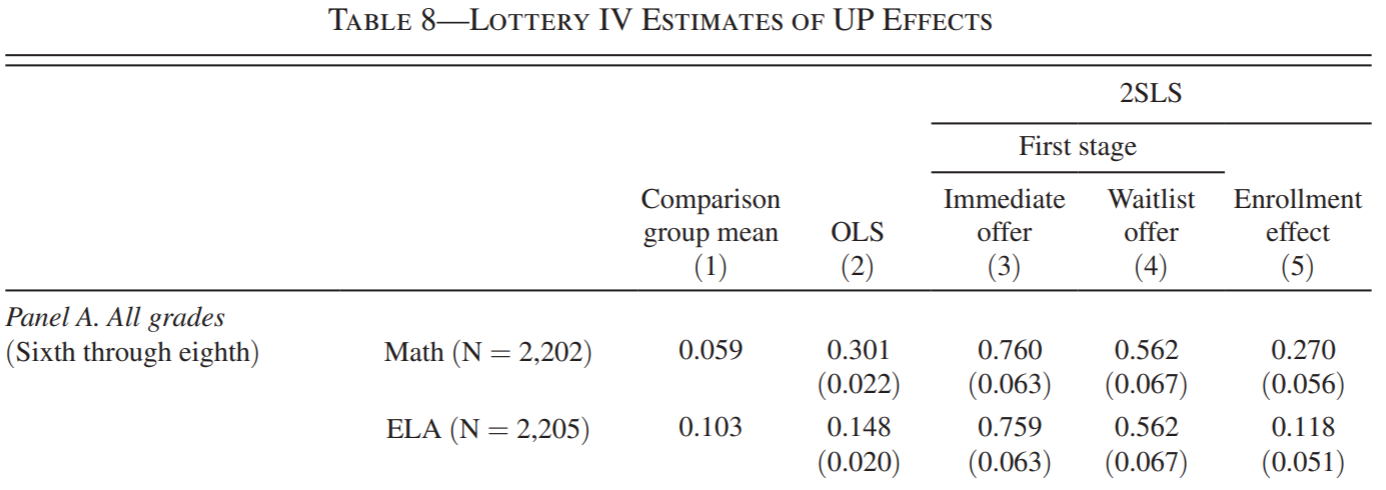
\includegraphics[scale=0.32]{./lecture_includes/charters1.png}
\end{center}

\end{frame}

\subsection{Natural Experiments}
\begin{frame}{Where do IVs Come From?}{2. Natural Experiments}
Without appealing to literal randomization, we may credibly argue $Z_i$ is as-good-as-randomly assigned conditional on some $\mathbf{W}_i$
\begin{itemize}
  \item Such ``natural experiments'' rely on a selection-on-observables argument (for $Z_i$, instead $D_i$)

  \item Still worry about exclusion: $Z_i$ cannot affect $Y_i$ except through $D_i$
\end{itemize}
\end{frame}

\begin{frame}{Example}{Quarter-of-Birth}
Angrist and Krueger (1991) famously estimate labor market returns to schooling with a creative IV: student quarter-of-birth

\begin{itemize}
  \item Compulsory schooling requirements prevent students from dropping before the day they turn 16 (used to be more binding)

  \item Fixed school start dates mean students who drop out at 16 get more or less schooling depending on their birth date\pause

  \item Quarter-of-birth seems quasi-randomly assigned --- is it excludable? See Buckles and Hungerman (2013)...
\end{itemize}
\end{frame}

\begin{frame}{The Quarter-of-Birth Natural Experiment: Visualized}

\vspace{-0.5cm}
\begin{center}
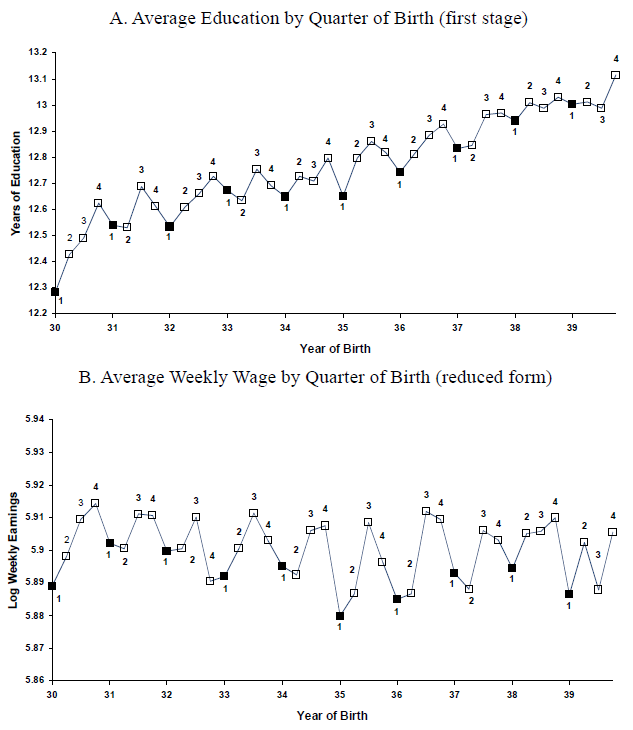
\includegraphics[scale=0.45]{./lecture_includes/qob1.png}
\end{center}

\end{frame}

\begin{frame}{Quarter-of-Birth IV Estimates of Returns to Schooling}

\begin{center}
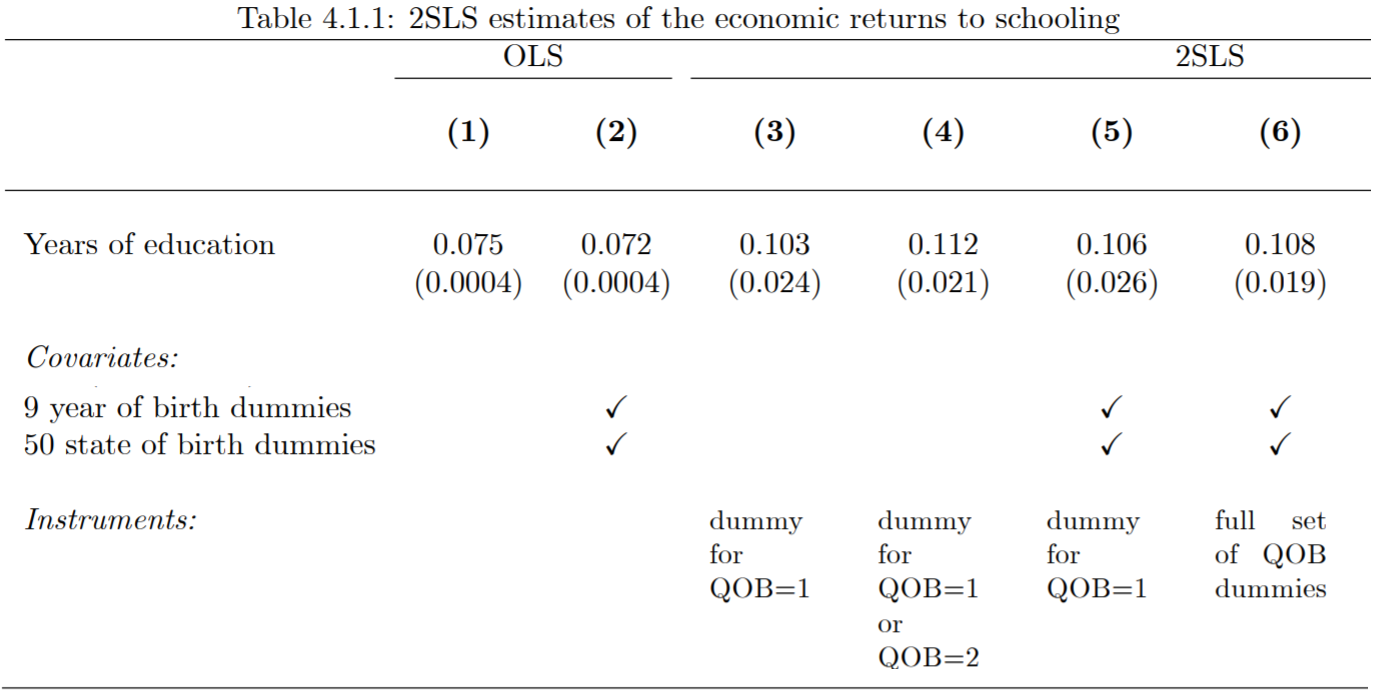
\includegraphics[scale=0.32]{./lecture_includes/qob2.png}
\end{center}

\end{frame}

\subsection{Panel Data}
\begin{frame}{Where do IVs Come From?}{3. Panel Data}

We might also combine IV + difference-in-differences identification
\begin{itemize}
  \item E.g. instrument with $Z_i\times Post_t$, controlling for $Z_i$ and $Post_t$ FEs

  \item This requires two parallel trends assumptions, for the RF and FS

  \item Still need to worry about the exclusion restriction, as always
\end{itemize}
\end{frame}

\begin{frame}{Example}{Charter School Takeovers}
Abdulkadiroglu et al. (2016) complement their lottery analysis of takeover charters with an instrumented diff-in-diff analysis
\begin{itemize}
  \item Students enrolled in the ``legacy'' public school were eligible for being ``grandfathered'' into UP, without having to apply to the charter

  \item We compare their trends in test scores \& enrollment to a matched comparison group of observably-similar students at other schools
\end{itemize}
\end{frame}

\begin{frame}{Grandfathering IV: Visualized}

\vspace{-0.2cm}
\begin{center}
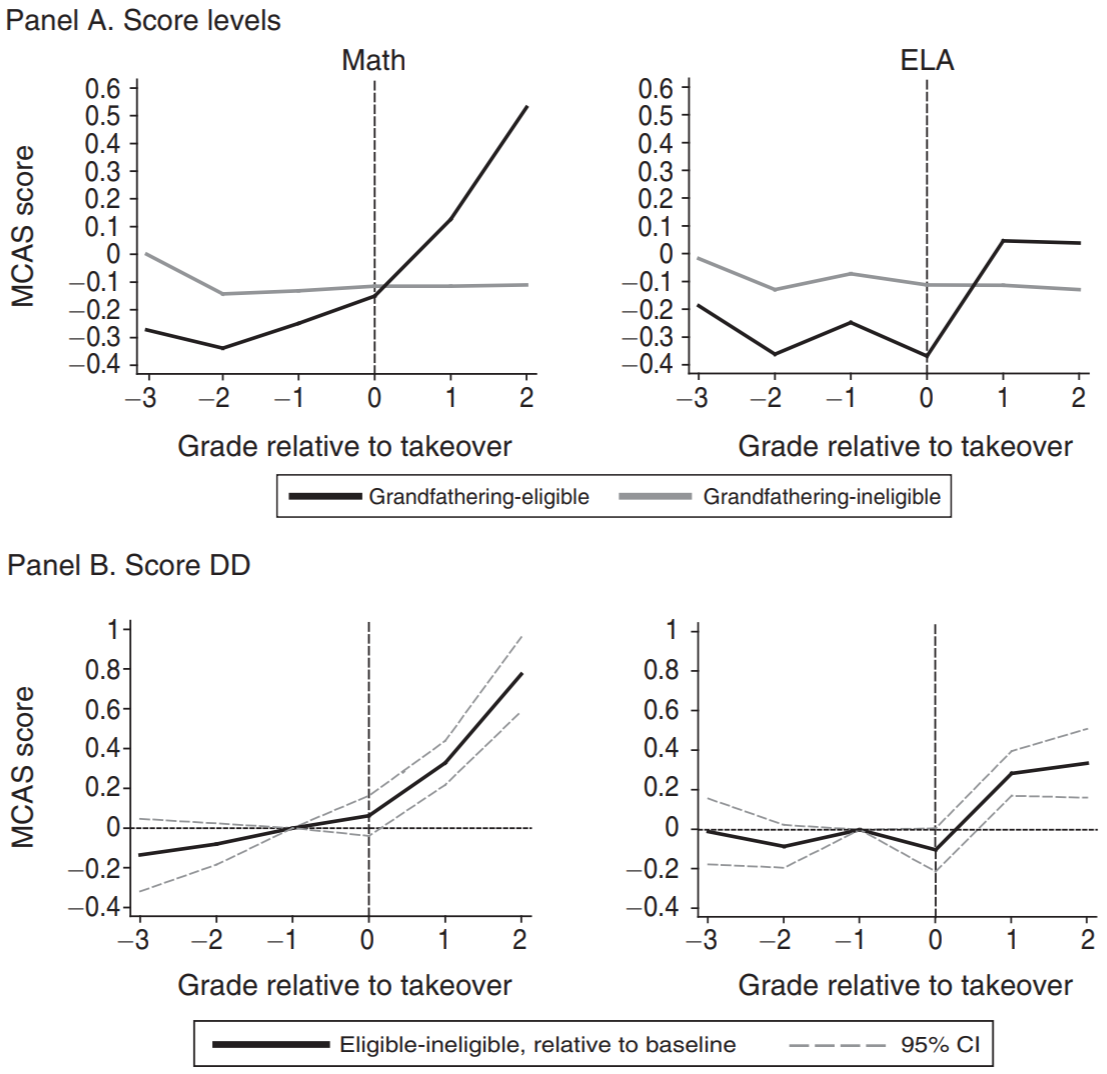
\includegraphics[scale=0.29]{./lecture_includes/charters2.png}
\end{center}

\end{frame}

\begin{frame}{Grandfathering IV Estimates of UP Test Score Effects}

\begin{center}
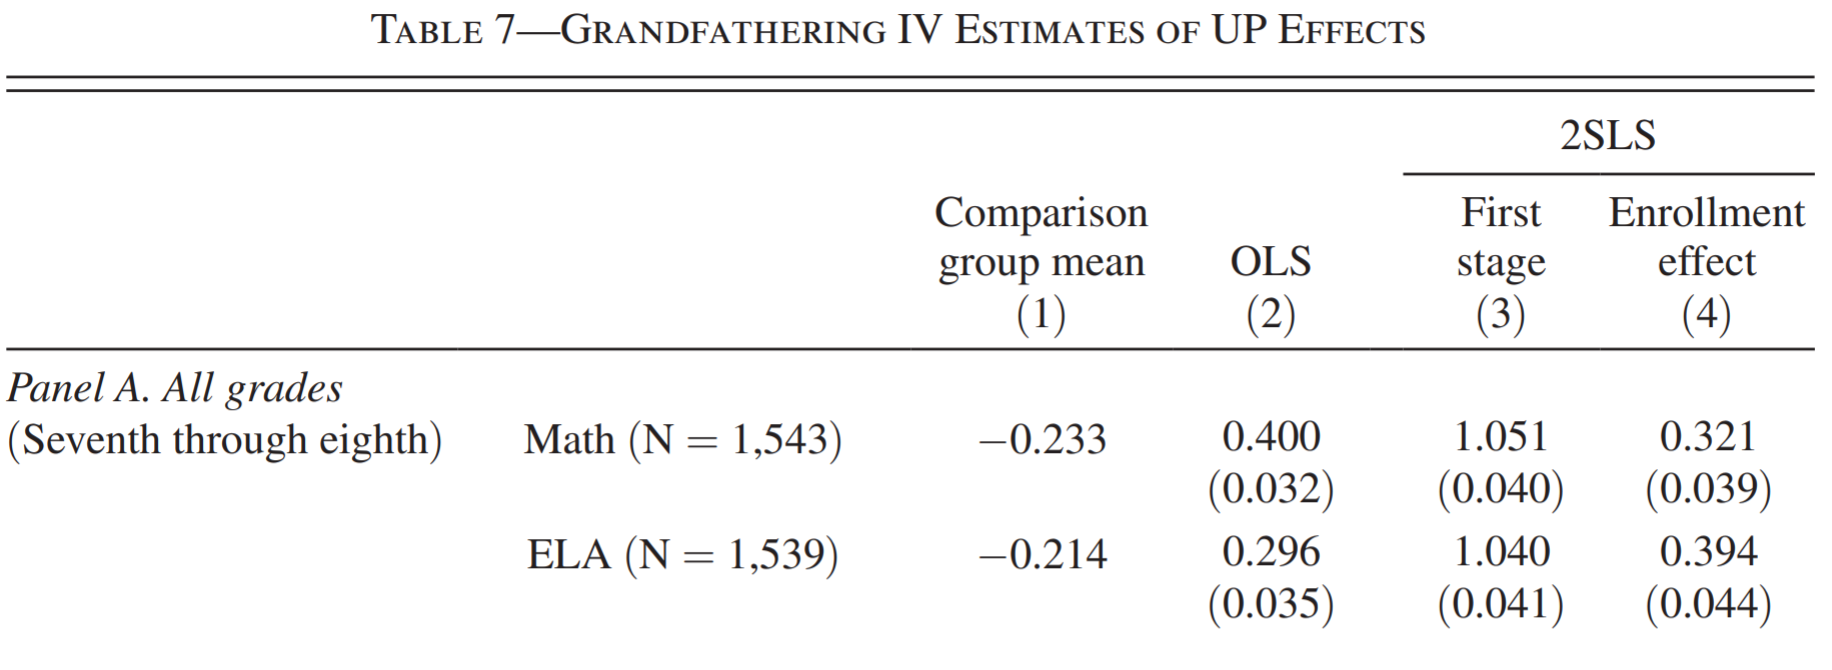
\includegraphics[scale=0.25]{./lecture_includes/charters3.png}
\end{center}

\end{frame}

\section{2SLS Mechanics}

\subsection{Just-Identified IV}
\begin{frame}{Just-Identified IV}

Tthe Stata \code{ivregress}/\code{ivreg2} commands (or \code{fixes::feols} in R) allows for controls and multiple treatments / instruments
\begin{itemize}
  \item When \# treatment = \# instruments, we say the IV is ``just-identified'':
\end{itemize}\pause\vspace{-0.7cm}

\begin{align*}
Y_i &=  \beta D_i +\mathbf{W}_i^\prime\boldsymbol{\gamma} +  \varepsilon_i\hspace{0.2cm}\text{(second stage)}\\
X_i &= \pi Z_i + \mathbf{W}_i^\prime\boldsymbol{\mu} + \eta_i\hspace{0.2cm}\text{(first stage)}
\end{align*}
where $\mathbf{W}_i$ includes a constant.
\end{frame}

\begin{frame}{Just-Identified IV}
The reduced form is: $$Y_i= \rho Z_i + \mathbf{W}_i^\prime\boldsymbol{\kappa}+\nu_i $$\pause
Same identification logic as before:

\begin{itemize}
  \item Validity: $Cov(Z_i,\varepsilon_i)=0$, allowing $Cov(Z_i,\mathbf{W}_i)\neq 0$\pause
  \item Relevance: $\pi\neq 0$, so $Z_i$ and $D_i$ are correlated controlling for $\mathbf{W}_i$
\end{itemize}\pause\medskip

IV is still ``reduced form over first stage'': ($\beta^{IV}=\rho^{OLS}/\pi^{OLS}$)\pause\vspace{0.1cm}
\begin{itemize}
  \item Can use Frisch-Waugh-Lovell to ``partial out'' $\mathbf{W}_i$ from $Y_i$, $X_i$, $D_i$, \\ and so get back to an IV regression without controls
\end{itemize}
\end{frame}

\subsection{Overidentification}
\begin{frame}{Overidentification}
Sometimes we have more than one instrument $Z_{i\ell}$, for $\ell=1,\dots,L$. This leads to an ``overidentified'' IV regression:

\vspace{-1cm}
\begin{align*}
Y_i &=  \beta D_i +\mathbf{W}_i^\prime\boldsymbol{\gamma} +  \varepsilon_i\hspace{0.2cm}\text{(second stage)}\\
X_i &= \mathbf{Z}_i^\prime\boldsymbol{\pi} + \mathbf{W}_i^\prime\boldsymbol{\mu} + \eta_i\hspace{0.2cm}\text{(first stage)}
\end{align*}
where $\mathbf{Z}_i=[Z_{i1},\dots,Z_{iL}]^\prime$. Reduced form: $Y_i= \mathbf{Z}_i^\prime\boldsymbol{\rho} + \mathbf{W}_i^\prime\boldsymbol{\kappa}+\nu_i $\pause

Validity: $Cov(Z_{i\ell},\varepsilon_i)=0$ for all $\ell$
\begin{itemize}
  \item ``Overidentified'' b/c we could use any $Z_{i\ell}$ to identify $\beta=\boldsymbol{\rho}_\ell/\boldsymbol{\pi}_\ell$\pause
  \item Relevance: $\boldsymbol{\pi}_\ell\neq 0$ for at least some $\ell$
\end{itemize}\pause\medskip

Overidentification can yield tests of IV validity
\begin{itemize}
  \item Intuitively, 2SLS checks whether all the $Z_{i\ell}$ yields the same IV estimate, which is sensible in a constant-effects model...
\end{itemize}
\end{frame}

\begin{frame}{Putting the ``2S'' in ``2SLS''}

You'll notice I haven't actually defined 2SLS beyond the simple case
\begin{itemize}
  \item Before we had $\beta^{IV}=\frac{Cov(Z_i,Y_i)}{Cov(Z_i,D_i)}$ leading to $\widehat\beta^{IV}=\frac{\widehat{Cov}(Z_i,Y_i)}{\widehat{Cov}(Z_i,D_i)}$ 
  \item General form follows similarly (as a sample analog) but is notation-heavy, so we won't go into it here
\end{itemize}
\pause

A more useful way to define 2SLS is by a two-step procedure:
\begin{itemize}
  \item First regress $D_i$ on all instruments $Z_{i\ell}$ and controls $W_{ik}$
  \item Then regress $Y_i$ on the ``fitted values'' $\widehat{D}_i$ and controls $W_{ik}$ 
\end{itemize}
\pause

The proof of this follows from some (simple) linear algebra 
\begin{itemize}
  \item Intuitively, regressing $Y_i$ on $\widehat{\pi}^{OLS}Z_i$ gives a scaled RF: 
  $$\widehat\beta^{IV}=\frac{\widehat{\rho}^{OLS}}{\widehat{\pi}^{OLS}}$$
\end{itemize}
\end{frame}

\begin{frame}{Avoid Manual 2SLS!}

Although easy, you should never do such ``manual 2SLS'' yourself!
\begin{itemize}
\item Your point estimates will be right, but your SEs won't be!\smallskip
\item Also might forget to include some controls in the second stage, etc
\end{itemize}
\bigskip
Just let Stata/R do everything for you...
\end{frame}

\begin{frame}{2SLS Done Right }

\vspace{-0.35cm}
\begin{center}
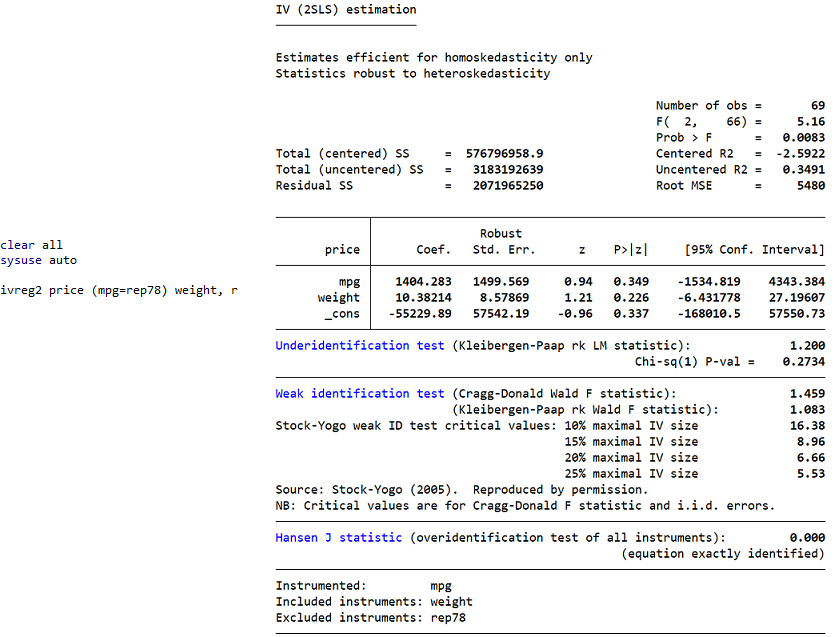
\includegraphics[scale=0.5]{./lecture_includes/auto_iv_results.png}
\end{center}

\end{frame}

\section{Weak and Many Instruments}

\subsection{Weak IV}
\begin{frame}{Weak Instruments}
\vspace{-0.2cm}

When running just-identified IV, you should always worry about the ``strength'' of your instrument
\begin{itemize}
  \item Specifically the first stage \bgPictonBlue{F-statistic}, which tests $\pi^{OLS}=0$ 
\end{itemize}
\smallskip\pause

If $\pi^{OLS}$ is small relative to its standard error, the IV is ``weak''
\begin{itemize}
  \item Typically use the rule-of-thumb of $\bgPictonBlue{F}<10$ (Staiger and Stock 1997)
  \item In this case the second-stage SEs will be large and the 2SLS estimate will tend to be biased towards the corresponding OLS
\end{itemize}\pause

Much made of this over the years, but Angrist and Koles\'{a}r (2022) argue recently that we shouldn't worry too much
\begin{itemize}
  \item The SE increase tends to be large enough to ``cover up'' the bias
  \item Just-id. 2SLS is ``approximately median-unbiased''
\end{itemize}

\end{frame}

\begin{frame}{Weak Instruments: Visualized}
\vspace{-0.2cm}
Monte Carlo: $Y_i=\varepsilon_i$, $D_i=\Pi Z_i+\eta_i$: $\Pi=Var(\varepsilon_i)=Var(\eta_i)=1$
\begin{center}
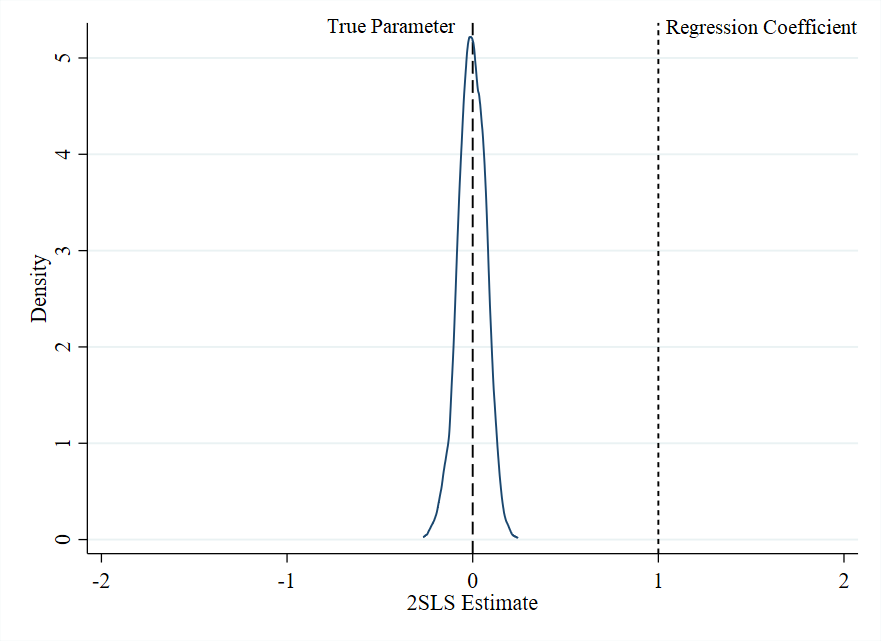
\includegraphics[scale=0.45]{./lecture_includes/strongpi.png}
\end{center}

\end{frame}

\begin{frame}{Weak Instruments: Visualized}
\vspace{-0.2cm}
Monte Carlo: $Y_i=\varepsilon_i$, $D_i=\Pi Z_i+\eta_i$: $\Pi=0.1$ (Weaker)
\begin{center}
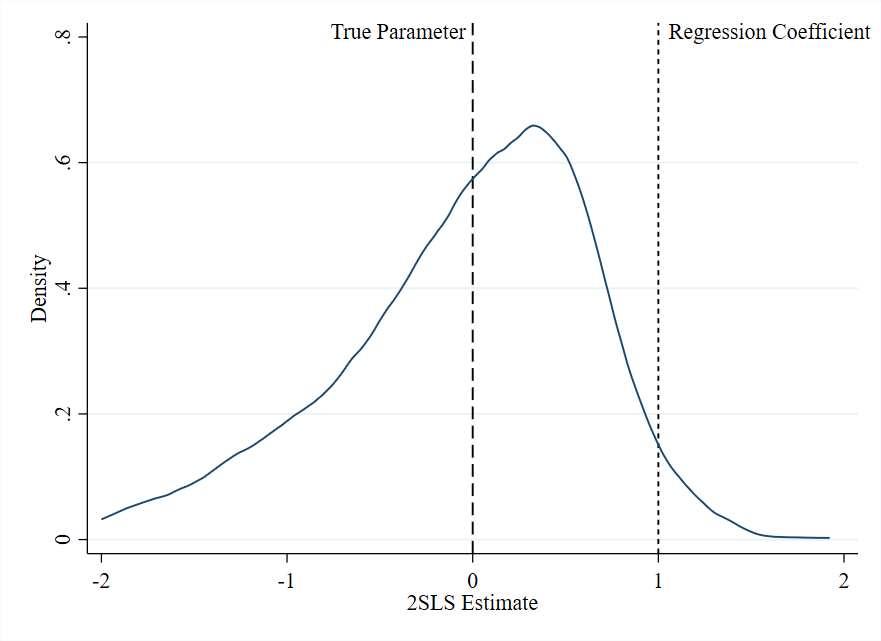
\includegraphics[scale=0.35]{./lecture_includes/medpi.png}
\end{center}

\end{frame}

\begin{frame}{Weak Instruments: Visualized}
\vspace{-0.2cm}
Monte Carlo: $Y_i=\varepsilon_i$, $D_i=\Pi Z_i+\eta_i$: $\Pi=0.01$ (Very Weak)
\begin{center}
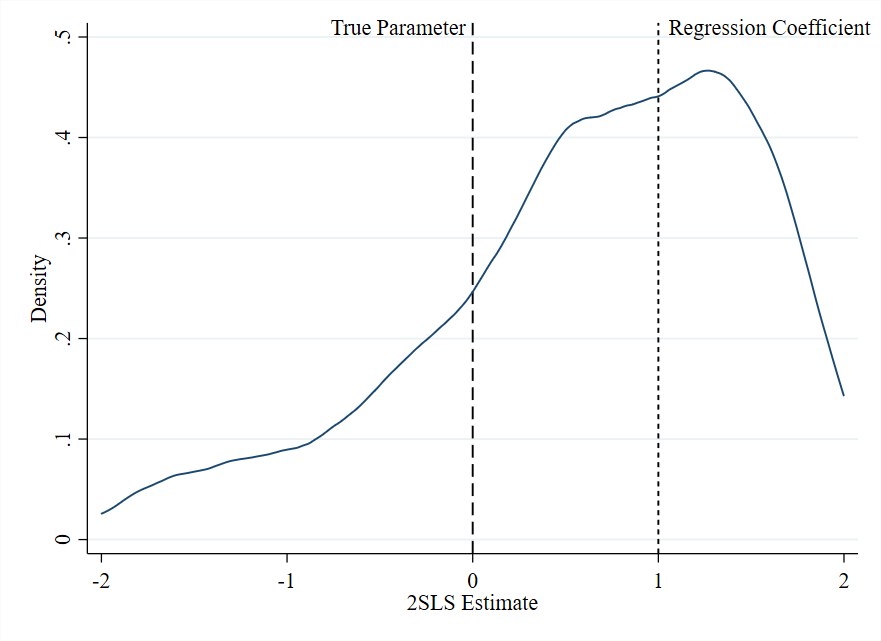
\includegraphics[scale=0.35]{./lecture_includes/weakpi.png}
\end{center}

\end{frame}


\subsection{Many IVs}
\begin{frame}{Many IVs}

A more pernicious problem is many-instrument bias, when overid\smallskip
\begin{itemize}
  \item Also tends to manifest in low first-stage F's, so also good to check
\end{itemize}\bigskip\pause{}

Many-IV bias is also towards OLS, but unlike before SEs go \emph{down}\smallskip
\begin{itemize}
  \item Intuitively, a more flexible FS tends to fit $D_i$ better $\rightarrow$ more power\smallskip
  \item But we can have \emph{overfitting} with lots of $Z_i$ $\rightarrow$ essentially recreate $D_i$
\end{itemize}\bigskip\pause{}

As we'll see, this bias is especially relevant in judge IV designs\smallskip
\begin{itemize}
  \item Potentially many judge assignment indicators as the instrument\smallskip
  \item Leave-out corrections (e.g. Angrist et al. 1999) have been adapted to this setting in recent years (e.g. Koles\'{a}r 2013)
\end{itemize}

\end{frame}

\begin{frame}{Weak and Many Instruments VIII}
\vspace{-0.2cm}
Monte Carlo: $Y_i=\varepsilon_i$, $X_i=\Pi Z_{i1}+\eta_i$: IV with one $Z_{i1}$
\begin{center}
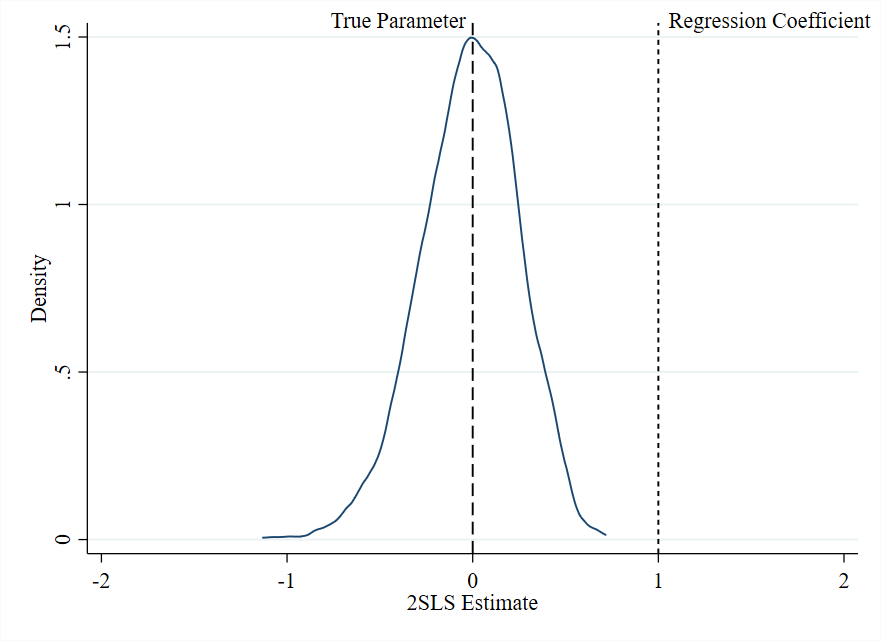
\includegraphics[scale=0.35]{./lecture_includes/fewz.png}
\end{center}

\end{frame}

\begin{frame}{Weak and Many Instruments IX}
\vspace{-0.2cm}
Monte Carlo: $Y_i=\varepsilon_i$, $X_i=\Pi Z_{i1}+\eta_i$: IV with ten $Z_{ij}$
\begin{center}
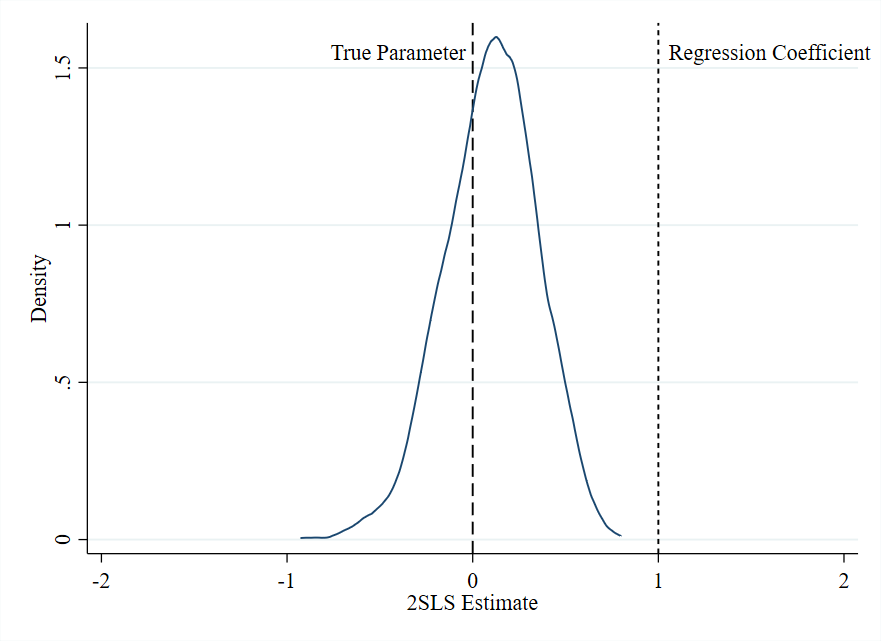
\includegraphics[scale=0.35]{./lecture_includes/somez.png}
\end{center}

\end{frame}

\begin{frame}{Weak and Many Instruments X}
\vspace{-0.2cm}
Monte Carlo: $Y_i=\varepsilon_i$, $X_i=\Pi Z_{i1}+\eta_i$: IV with 100 $Z_{ij}$
\begin{center}
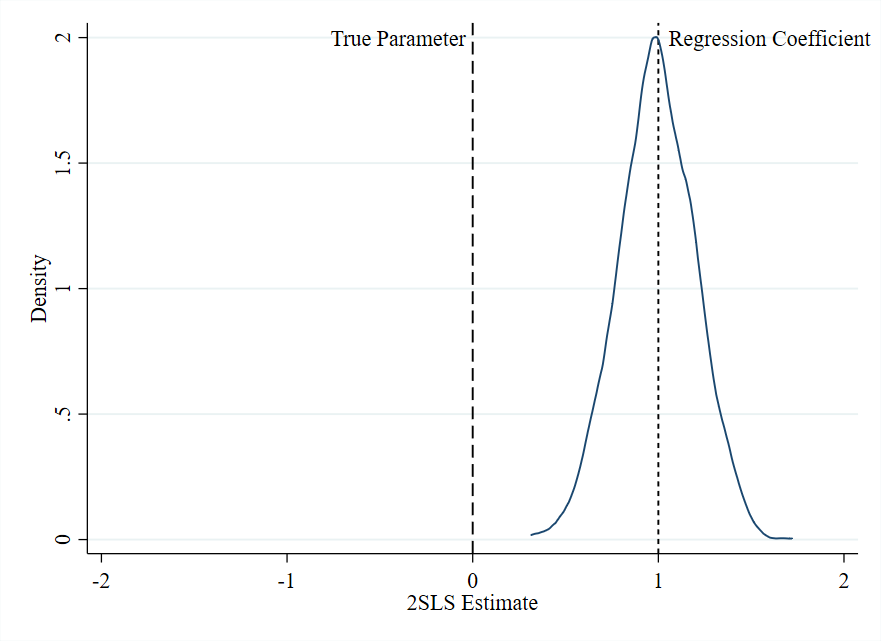
\includegraphics[scale=0.35]{./lecture_includes/manyz.png}
\end{center}

\end{frame}

\begin{frame}{What to Do?}
Check your F's after every IV regression\smallskip
\begin{itemize}
\item Staiger-Stock rule-of-thumb ($F>10$) still seems widely held\smallskip
\item See Lee et al. (2020) for a recent alternative approach
\end{itemize}
\bigskip

If your F is small, some things to consider:\smallskip
\begin{itemize}
\item Is there a different instrument that's stronger?\smallskip
\item Is there a better functional form for the instrument you have?\smallskip
\item Do interactions with covariates help? (note: beware many-weak!)\smallskip
\item Does changing the covariate set help? (note: beware invalidity!)
\end{itemize}
\end{frame}
\end{document}
